\section{Introduction}
The EuBIC-MS Developers Meeting is organized every other year by the European Bioinformatics Community for Mass Spectrometry (EuBIC-MS, eubic-ms.org), an initiative of the European Proteomics Association (EuPA) for user-oriented bioinformatics. EuBIC-MS promotes the use of bioinformatics for mass spectrometry (MS). Our goal is to bring together the European MS bioinformatics community, including students, early-career researchers, and long-standing experts from academia and industry. Through the setup of community-driven initiatives, EuBIC-MS mainly focuses on improving education in computational methods, highlighting job and funding opportunities, promoting international collaborations, publications of specialized studies, and training in specialized software tools. To this end, EuBIC-MS maintains, in collaboration with EuPA, several web resources that include educational videos, grant overviews, a job fair, and tutorials, all available on www.proteomics-academy.org. Besides these online resources, EuBIC-MS regularly organizes workshops and hubs at major international conferences on MS and proteomics. Additionally, an annual conference on computational MS is organized by EuBIC-MS itself, forming an important community outreach effort to bring together bioinformatics researchers from all over Europe.

Since 2017, EuBIC-MS's Winter School takes place every two years \citep{pmid28385664}, (PMID: ?EuBIC2022?). These events are highly attended and are a unique opportunity to learn, discover new tools and methods, and discuss current challenges in the field. However, not all computational expertise is utilized to its full potential in a typical conference setup. Therefore, we alternate the Winter School every other year with a Developers Meeting, which targets software developers and computation-aware end-users. The first official Developers Meeting occurred in Ghent, Belgium, in 2018 \citep{pmid29864591} and Nyborg, Denmark in 2020 \citep{EuBIC-MS2020}. This year's meeting was held at the Congressi Stefano Franscini on Monte Verità in Ticino, Switzerland, from January 15th to January 20th, 2023. A total of 58 participants, including keynote speakers, participated in the meeting (for more statistics see Table~\ref{tab:stat}). It took off with five keynotes and a poster flash talk session where 26 participants gave a 60-seconds `elevator pitch' on their poster. In the next four and a half days, the participants split up into seven teams to each work on a project that was proposed and selected through an open call and selection process \href{https://github.com/eubic/EuBIC2023/issues}{eubic/EuBIC2023/issues}. On the final day, we showcased two sponsor presentations and unveiled the output from the hackathons. Additionally, we announced the winner of the best poster. This meeting, organized by and for the European computational MS community, provided a unique opportunity to learn, network, and participate in developing promising tools. The detailed program is available on \url{https://eubic-ms.org/events/2023-developers-meeting}.

\begin{figure*}[h]
\centering
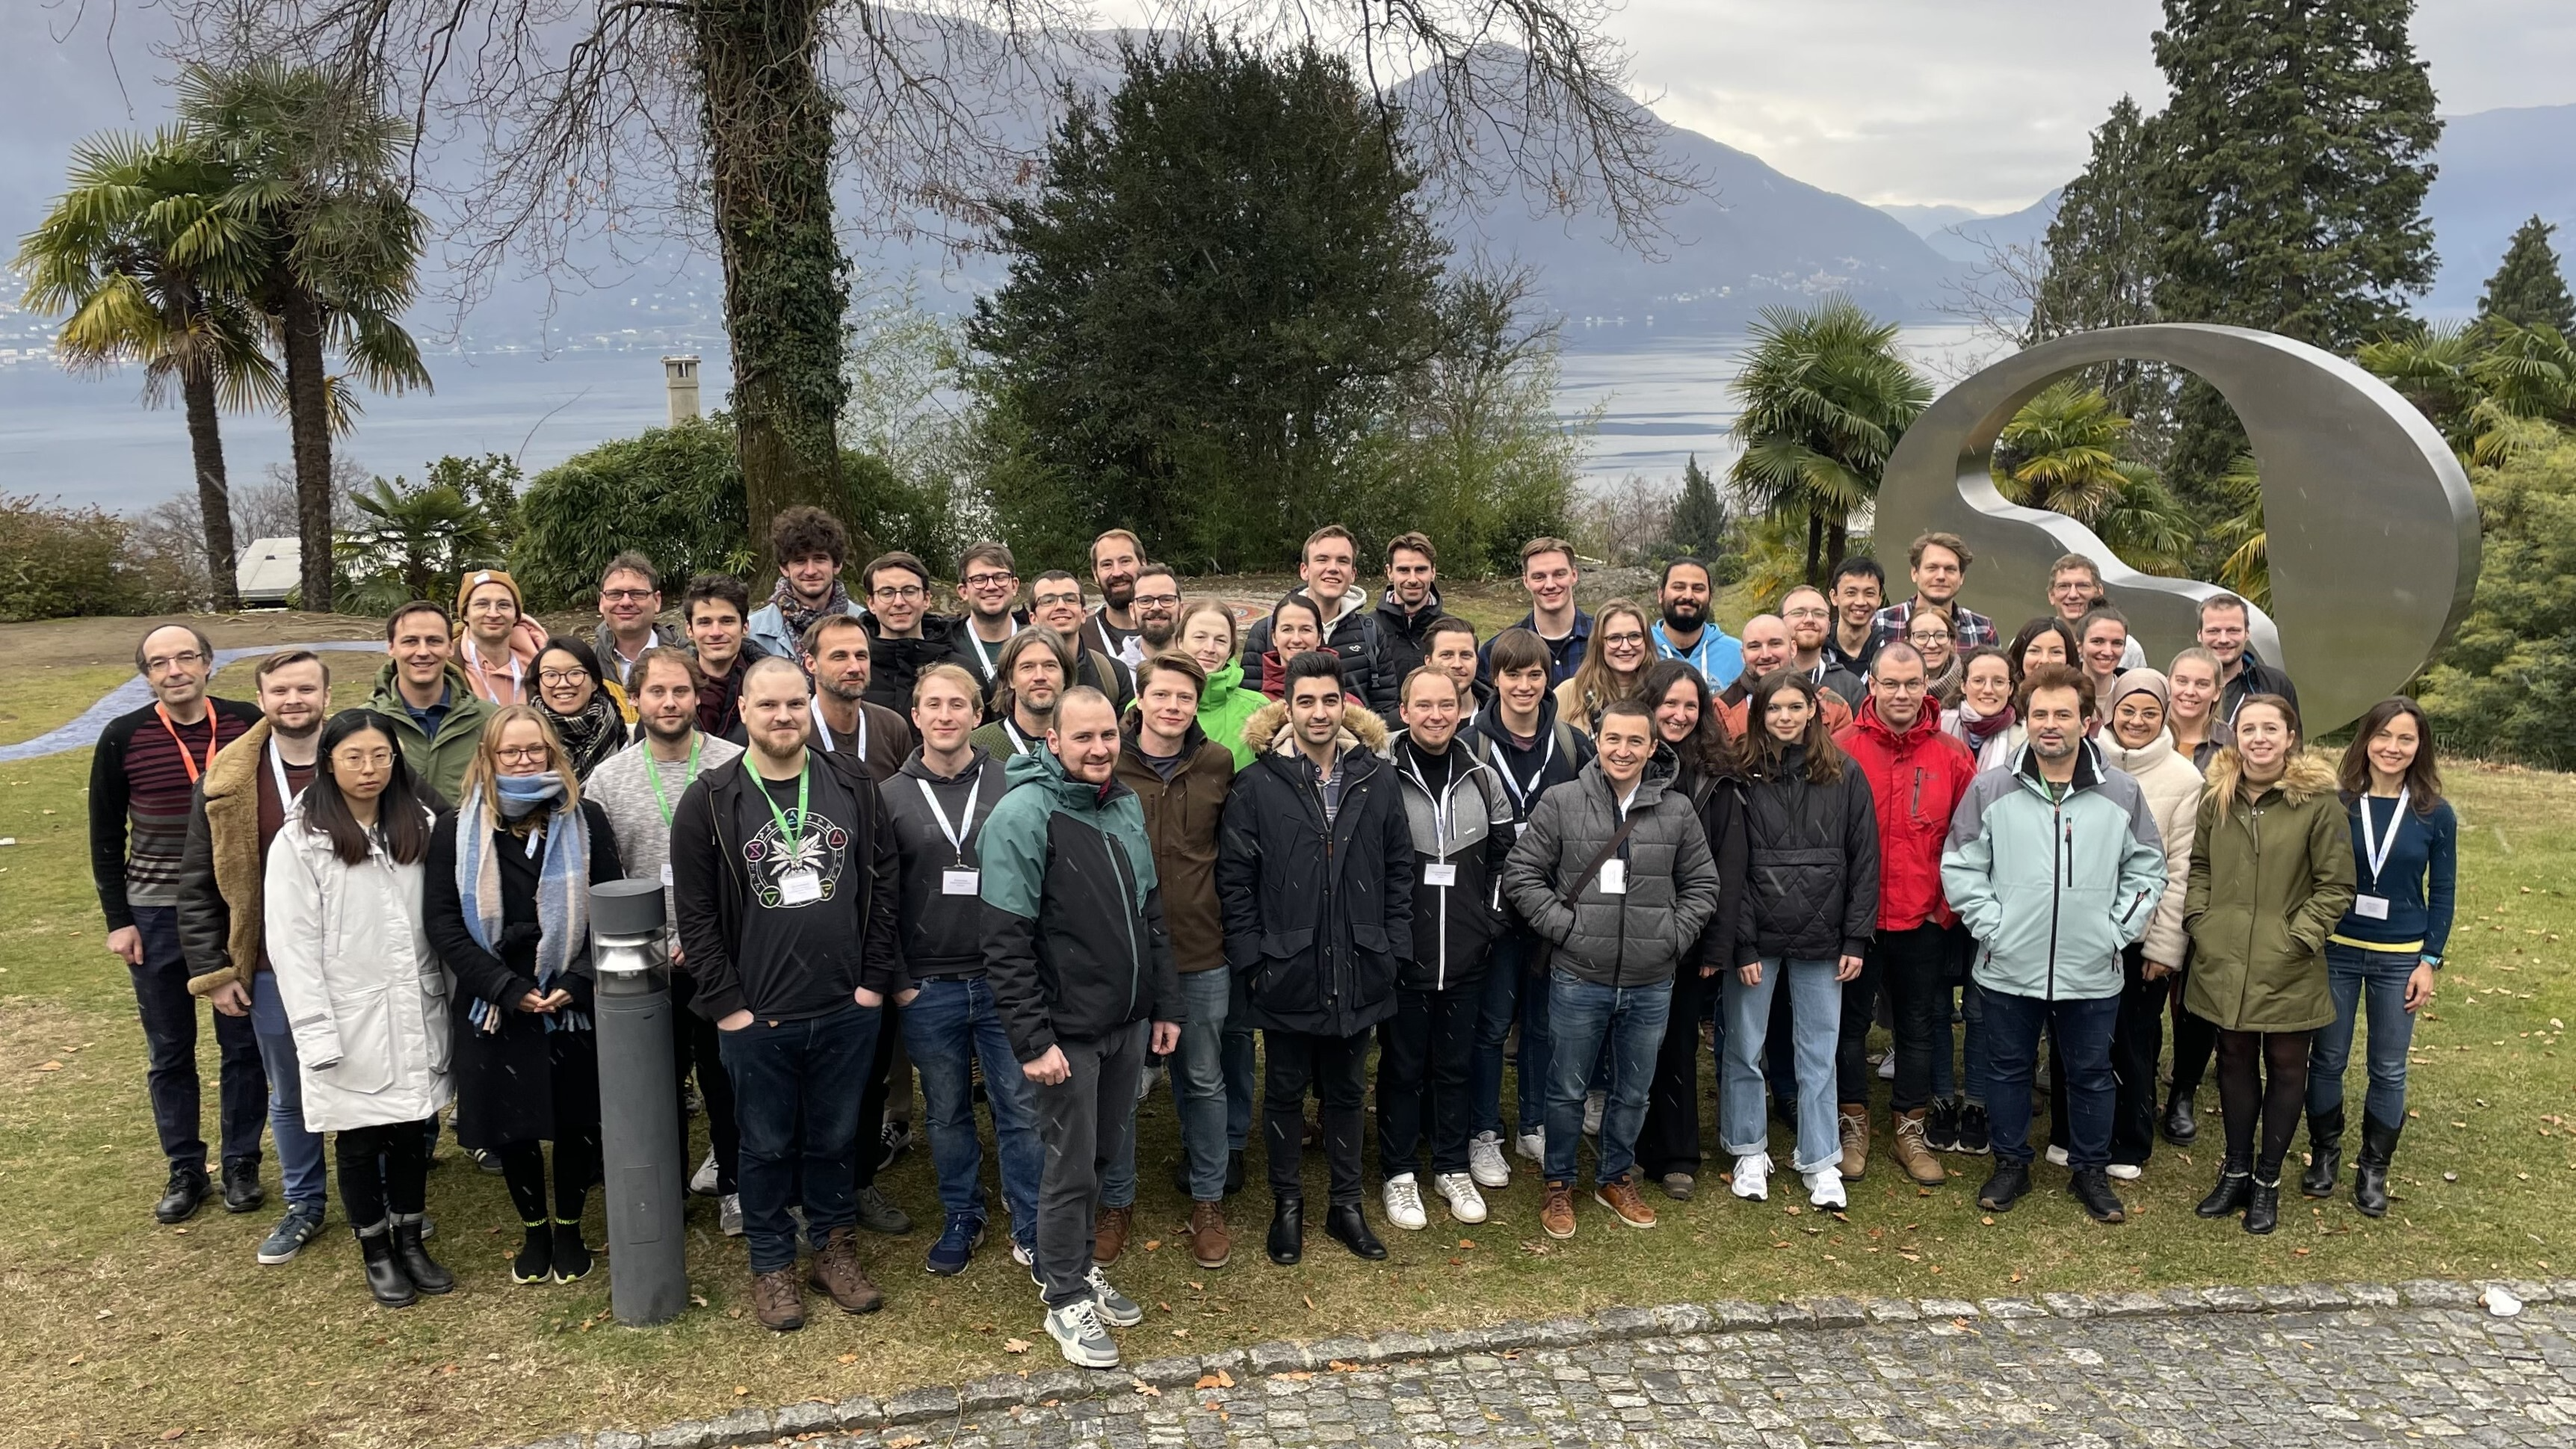
\includegraphics[width=1.0\textwidth]{images/EuBICMS2023}
\caption{Participants of the EuBIC-MS Developers’ Meeting 2023 on Monte Verità 322NN, Ticino, Switzerland. source: \url{https://twitter.com/kusterlab/status/1614974632569749504}}
\end{figure*}

\begin{table}
\centering
\label{tab:stat}
\begin{tabular}{ll}
\hline
location	&	\href{https://en.wikipedia.org/wiki/Monte_Verit%C3%A0}{Monte Verità, CH}\\	
duration	&	$5$ days\\
\#participants	&	$58$\\
\#keynotes	&	$5$\\
\#hackathons	&	$7$\\
\#posters	&	$26$\\
\#percentage female&	$>25\%$\\
\#institutions	&	$25$\\
\#EU countries&	$>10$\\
\#sponsors	&	$4$\\
\hline
\end{tabular}
\caption{Statistics of the meeting}
\end{table}
